% Chapter 3



%TODO: MarginPARS zetten
\chapter{Onderzoeksmethode}\label{ch:onderzoeksmethode} % Chapter title

Op basis van de requirements analyse beschreven in het vorige deel zijn er een aantal vragen ontstaan die verder onderzoek benodigd behoeven. In dit deel worden de vragen geanalyseerd en beantwoord zodat er een duidelijkheid is in de materie en een goede basis wordt gelegd voor de daadwerkelijke implementatie beschreven in het volgende deel. Er is gekozen om het vooronderzoek in drie hoofdstukken op te delen omdat ieder deel onderzoek een eigen uitgesproken onderwerp heeft. Zeker het onderzoek naar de manier van werken binnen EagleScience staat in zeker los van de thee hoofdstukken over cybersecurity en later over methodes om bibliotheken te analyseren. Echter is de informatie die het resultaat is van het ene onderzoek input voor het onderzoek erna. Door eerst te kijken naar de manier waarop Eaglescience werkt kan die als een scope dienen voor de onderzoeken die er na uitgevoerd worden.

Om verder inzicht te krijgen in de materie rondom de opdracht is er onderzoek nodig. Er worden drie onderzoek gedaan die ieder zijn eigen onderwerp hebben. Gezamelijk zorgen ze voor input voor het ontwerp en de daadwerkelijke implementatie. In dit hoofdstuk word ingegaan op de manier waarop de onderzoeken zijn uitgevoerd en welk doel zei hebben. Daarna volgt er voor ieder onderzoek een eigen hoofdstuk die het onderwerp behandeld en met resultaten komt. Als laatst is er een algehele conclussie die als input dient voor het ontwerp van de implementatie.

\section{Scope}
Het onderzoek zal zich beperken tot de benodigde informatie voor het implementeren van de nieuwe oplossing voor een geautomatiseerde SOUP analyse.
Het zal ingaan op de gebruikte ontwikkelstack binnen Eaglescience en bestaande architectuur gezien de nieuwe oplossing een onderdeel is van een al bestaand project en hier dus naadloos op moet integreren.
Daarnaast zal er onderzoek gedaan worden naar wat een SOUP-analyse daadwerkelijk is en welke problemen het mogelijk op kan lossen.
Met daarbij een mogelijke oplossingen om een SOUP analyse te kunnen doen.

Gezien de vragen in twee verschillende domeinen gesteld worden is het ook noodzakelijk om deze vragen op te delen in twee onderzoeken.
In de komende hoofdstukken zal er dan ook voor ieder domein een eigen onderzoek worden beschreven met daarin de resultaten die vervolgens gebruikt kunnen worden voor de implementatie die volgt in een volgend deel.
\section{Onderzoek 1: Literatuur studie Noodzaak van SOUP analyse}\label{sec:onderzoek:-literatuur-studie-soup}
[NOTE: Vraag me af of dit onderzoek nog nodig is apart te onderzoeken. ]
\textBF{Doel: } Algemene inzichten onderzoeken op het gebied van Software veiligheid en het nog veiliger maken van diezelfde software.

\textbf{Methode: }

\begin{figure}[h!] %Todo: Nog in kleur zetten van Eaglescience als deze goed is.
  \myfloatalign
  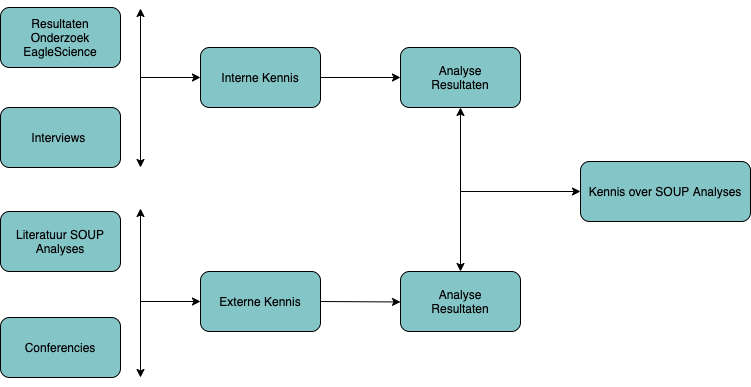
\includegraphics[width=10cm]{gfx/OnderzoeksmodelSOUP}
  \caption{Onderzoeksmodel SOUP analyse module}
  \label{fig:OnderzoeksModelNoodZaakSOUP}
\end{figure}
\textbf{Bronnen: }

Dit onderzoek is vooral bedoeld om wegwijs te raken in de wereld het zoeken naar kwetsbaarheden binnen externe bibliotheken.
Het gaat voornamelijk in op de betekenis van de verschillende begrippen en vervolgens hoe belangrijk het is om deze analyse uit te voeren.
De uitkomst van dit onderzoek is een basis kennis die als entree voor de komende onderzoeken gebruikt kan worden.
Het onderzoek heeft niet echt een hoofdvraag waardoor er een duidelijke scope moet worden gedefineerd.
De volgende zaken moet duidelijk worden in dit onderzoek:
\begin{itemize}
  \item "Wat is SOUP?"
  \item "Waarom kan het gebruik van SOUP gevaarlijk zijn?"
  \item "Hoe worden deze gevaren/kwetsbaarheden gelogd?"
  \item "Wat is een CVE en een CVSS?"
\end{itemize}


\section{Onderzoek 2: Architectuur binnen Eaglescience}\label{sec:onderzoeksmethode-architectuur-binnen-eaglescience}
Een intern onderzoek om kennis te vergaren in de manier waarop software wordt ontwikkeld en uitgerold.

\textbf{Doel: }Het doel van dit onderzoek is inzicht te krijgen in de manier waarop EagleScience software ontwikkeld en op welke manier deze uitgerold wordt. Deze kennis is relevant omdat de module die ontwikkeld dient te worden binnen deze manier moet passen zonder dat er grote aanpassingen gedaan dienen te worden aan de werkwijze.

\textbf{Methode: } Om de resultaten te verkrijgen dient er een deskreseach gedaan te worden met als input de documenten die door EagleScience beschikbaar gesteld zijn met als extra input verschillende gesprekken die gevoerd zijn met collega's die langer werkzaam zijn.

\begin{figure}[h!] %todo: Nog in kleur zetten van Eaglescience als deze goed is.
  \myfloatalign
  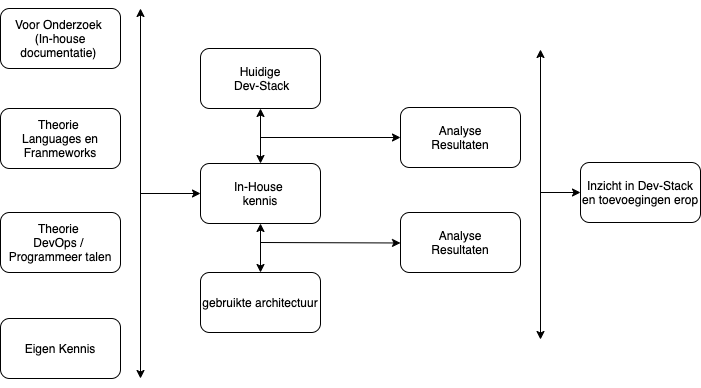
\includegraphics[width=10cm]{gfx/OnderzoeksmodelES}
  \caption{Onderzoeksmodel Eaglescience}
  \label{fig:OnderzoeksModelEaglescience}
\end{figure}

\textBF{Bronnen: } De bronnen die voornamelijk gebruikt worden zijn interne documenten waarin vermeld staat hoe een project verloopt en welke tooling er gebruikt wordt. Daarnaast zal er veel gebruik gemaakt worden van kennis van collega's.



\section{Onderzoek 3"  Implementatie van een SOUP-analyse}\label{sec:onderzoek-naar-soup-analyse}
\textBF{Doel: } Het doel is om een methode te vinden welke gebruikt kan worden om een SOUP-analyse te doen binnen de architectuur van EagleScience. De mtehode moet een output leveren die voor iedereen binnen EagleScience te begrijpen is.

\textbf{Methode: } Een zoektocht naar applicaties en/of plugins die in staat stellen om de dependencies van een project te analyseren. Een
selectie te maken van

\textbf{Bronnen: }
\begin{figure}[h!] %Todo: Aanpassen aan het onderzoeksmodel van SOUP analyse
  \myfloatalign
  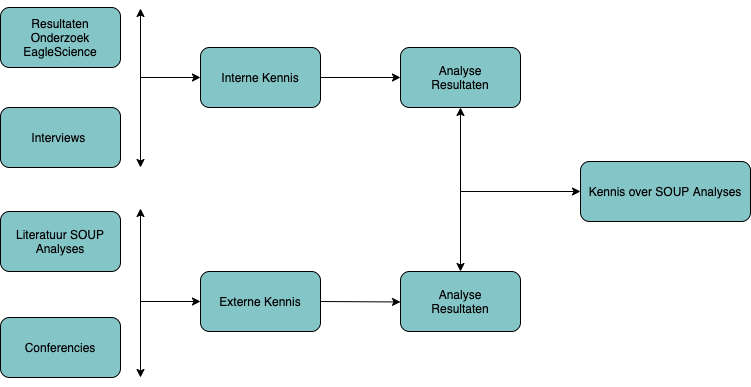
\includegraphics[width=10cm]{gfx/OnderzoeksmodelSOUP}
  \caption{Onderzoeksmodel SOUP analyse module}
  \label{fig:OnderzoeksModelSOUPAnalyse}
\end{figure}

\textbf{Bronnen: }



Dit onderzoek heeft als ingang het gegeven dat er kwetsbaarheden in de bibliotheken zitten met daarbij de dev-stack van Eaglescience.
Het resultaat van dit onderzoek moet zijn dat er een methode moet zijn waarbij er een assesment op de bestaande dev-stack binnen de werkwijze van Eaglescience moet komen die geimplementeerd kan worden.
Het onderzoekmodel (figuur:\ref{fig:Onderzoeks model Dev-Stack}) geeft weer dat de ingangs kennis de opgedane kennis uit het onderzoek naar de architectuur van Eaglescience en een literatuur studie naar mogelijkheden om soup te analyseren.
Veel kennis van buiten zal worden vergaard door middel van het lezen van artikelen en boeken over het onderwerp.
Hierbij moet worden gelet op de toepasbaarheid en scope van het artikel.
